\scanpage{27}
\uline{Cas particulier} Celui où $(xy)(zt)=0$ quels que soient $x,y,z,t$, i.e.
\margin{[i.e. $(H^1)\unsure{H^3|(H^1)^3}=0$ dans $H^4$ !]}
si l'image de $\alpha:\bigwedge^2V\longrightarrow k\xi+W$ est \deleted{\unsure{dans}} \unsure{un} ss-espace isotrope de $k(\xi)+W$.
\deleted{\unsure{Par exemple si} $W\unsure{\neq0}$, \unsure{dans le cas alg. clos cela se réalise néc. ainsi :} si $W$ est \inserted{de dim} (\unsure{impaire}), alors on peut}

$Q$ non dég. \unsure{étant donné}, et supposons $W\neq0$, il existe (si $k$ \deleted{\unsure{ensuite}} alg. clos disons) une droite isotrope $D$ dans $k\xi+W$ qui n'est pas dans $W$, et on prendra pour $\alpha$ \deleted{\unsure{une forme}} définie par une \deleted{forme}\inserted{appl.} bilinéaire \inserted{alt.} non dégénérée \deleted{\unsure{sur}} de $V\times V$ dans $D$: alors $\varphi$ sera aussi non isotrope\ldots

\figure{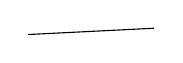
\begin{tikzpicture}\draw (0,0)--(1.6,0.08);\end{tikzpicture}}

Plus généralement, considérons la forme 4-linéaire alternée $\chi$ définie par
\[
xyzt=\chi(x,y,z,t)\xi^2\qquad(x,y,z,t\in V)
\]
Alors la forme \inserted{bilinéaire} induite par la \inserted{forme} $Q\oplus1$ (sur $k\xi+\unsure{V|W}$) sur $\bigwedge^2 V$ par $\alpha$, qui définit une \deleted{forme} forme linéaire sur
\diagram{\begin{tikzcd}[ampersand replacement=\&,column sep=large]
\operatorname{Sym}^2(\bigwedge^2V)\arrow[rr,bend right=18,"\unsure{épi.}"']\&\text{, se factorise en}\&\bigwedge^4V
\end{tikzcd}}
moyennant $\chi$, et donc les données sont les suivantes

a) $V$ vect. (de dim finie) sur $k$

\deleted{b) $\varphi:\bigwedge^2V\longrightarrow k$}

b) $\chi:\bigwedge^4V\longrightarrow k$, définissant une forme bilinéaire symétrique $\chi'$ sur $\bigwedge^2V$

c) un vectoriel $\widetilde W$, avec une forme \deleted{quadratique}\inserted{bil. sym.} $\widetilde Q$, et une application linéaire
\[
\bigwedge^2V\xrightarrow{\alpha}\widetilde W
\]
compatible avec $\chi',Q$ [on dira que $\widetilde W,\widetilde Q$ est une \uline{extension} de la forme $\chi'$]

d) un élément $\xi$ de $\widetilde W$, tel que $Q(\xi,\xi)=1$.

\uline{Condition de non dégénérescence}
\[
\left|\begin{array}{l}
Q\text{ non dégénérée}\\
\varphi(x,y)=Q(\alpha(xy),\xi)\text{ non dégénérée}
\end{array}\right.
\]
\mspage{26}
